\documentclass[twocolumn]{gwclass}
\usepackage[utf8]{inputenc}

\usepackage{tikz-cd}
\usepackage{amsthm}
\usepackage{graphicx}
\usepackage{wrapfig}
\usepackage{caption}
\graphicspath{{img/}}

\newcommand{\man}{\mathcal{M}}
\newcommand{\R}{\mathbb{R}}
\newcommand{\C}{\mathbb{C}}
\newcommand{\Z}{\mathbb{Z}}
\newcommand{\W}{\mathcal{W}}

\newcommand{\bt}[1]{\text{\textbf{#1}}}

\newcommand{\realE}{\*{\mathcal{E}}}
\newcommand{\realD}{\*{\mathcal{D}}}
\newcommand{\realB}{\*{\mathcal{B}}}
\newcommand{\realH}{\*{\mathcal{H}}}

\title{Electromagnetic Theory}
\author{--- George Willingham ---}
\date{}

\begin{document}
	\maketitle
	\tableofcontents
	\section{Microscopic Theory}
	\subsection{Point Charges \& The Field Concept}
	The foundational elements of electromagnetic theory are \emph{charges} and \emph{fields}. Charge is regarded as a fundamental property of matter and is the quantity that controls how strongly a bit of matter participates in electromagnetic interactions. It comes in two \emph{types}: there is positive and negative charge. Charges of the same type repel each other while opposite charges attract. The interaction between charges is mitigated by the \emph{electromagnetic field}. Indeed, it is not the case that one charge directly applies force to another. More truly a charge is the source of a field that permeates through all space and any other charge interacts with that field rather than with the charge directly. This might seem nit-picky, semantic, and inconsequential, but it becomes crucially important when dealing with dynamic systems. As a charge moves, the field it generates changes but that change propagates at a finite speed. Another charge on the other side of the universe will surely not feel a new field at the exact moment when the charge starts moving. This is all to say that fields are necessary to preserve \emph{locality}: the principle that causes and effects are spatially correlated.
	\subsection{Maxwell's Equations}
	All of electromagnetic theory is codified in five equations: Maxwell's equations and the Lorentz force law. There are the two divergence equations (Gauss' laws):
	\begin{align*}
		\nabla\cdot \*E &= \frac{\rho}{\epsilon_0}\\
		\nabla\cdot \*B &= 0
	\end{align*}
	Qualitatively, these equations tell us that the electric field $\*E$ has a charge density $\rho$ as its source and the magnetic field $\*B$ has no source, i.e. there are no magnetic charges. In the microscopic/fundamental theory, the charge density consists of all the point-charges in a system and we write
	$$ \rho(\*r,t) = \sum_i q_i \delta(\*r-\*r_i(t)) $$
	where $q_i$ is the charge of the $i^\t{th}$ particle and $\*r_i(t)$ is its position at time $t$.
	
	The divergence equations are often thought of as conditions that the E and B-fields must satisfy rather than equations that we seek to solve. The \emph{dynamical} Maxwell's equations which determine how the fields evolve in time are the curl equations:
	\begin{align*}
		\nabla\times\*E &= -\frac{\partial \*B}{\partial t}\\
		\nabla\times\*B &= \mu_0\*j + \epsilon_0\mu_0\frac{\partial \*E}{\partial t}
	\end{align*}
	The first equation is \textbf{Faraday's law} and the second is known as the \textbf{Maxwell-Ampere} law. These equations tell us that the electric and magnetic fields are tightly coupled --- the E-field determines how the B-field evolves and vice versa. This coupling will ultimately lead us to see that we should not (or even \emph{cannot}) treat electricity and magnetism as distinct phenomena. It turns out that whether you see only an E-field or a combination of E and B \emph{depends} on your reference frame. The fundamental quantity is the combined \emph{electromagnetic field}. 
	
	The current density, or \emph{charge flux}, $\*j$ is microscopically defined in terms of the motion of charged particles:
	$$ \*j(\*r,t) = \sum_i q_i\*v_i(t)\delta(\*r - \*r_i(t))$$
	where $\*v_i(t)$ is the velocity of the $i^\t{th}$ particle. Importantly, notice that if we take the divergence of the Maxwell-Ampere equation, Gauss' law leads us to the continuity equation:
	$$ \frac{\partial \rho}{\partial t} = -\nabla\cdot\*j $$
	So then, Maxwell's equations imply the local conservation of charge. Charge cannot be created or destroyed --- it can only move.
	
	Finally, we have the Lorentz force law which states that the force on a point particle with charge $q$ and velocity $\*v$ is 
	$$ \*F = q(\*E + \*v\times\*B) $$
	The dependence on velocity is hinting at relativistic effects that will be explored in a later section.
	
	\subsection{Electromagnetic Waves}
	There is a very useful vector calculus identity that allows us to simplify the curl of a curl. For any vector field $\*G$, we have $\nabla\times\nabla\times\*G = \nabla(\nabla\cdot\*G) - \nabla^2\*G$. 
	Armed with this, we can take the curl of the both of Maxwell's curl equations and then use Gauss' laws to arrive at a new form of Maxwell's equations:
	\begin{align*} 
		-\nabla^2\*E + \epsilon_0\mu_0\frac{\partial^2\*E}{\partial t^2} &= -\frac{\nabla\rho}{\epsilon_0} - \mu_0\frac{\partial \*j}{\partial t} \\
		 -\nabla^2\*B + \epsilon_0\mu_0\frac{\partial^2\*B}{\partial t^2} &= \mu_0\nabla\times\*j 
	 \end{align*}
	The left hand side is recognized as the wave operator so these are \emph{inhomogeneous wave equations}. Consequently this tells us that \textbf{electromagnetic waves} exist, i.e. free propagating waves in $\*E$ and $\*B$. Further, these waves are sourced by gradients in the charge density and circulating or otherwise time-variant currents. These equations are cumbersome to work with and are typically not used in practice, but they provide a nice intuitive picture of the physics at play. For instance, antennas work exactly by the physics in these equations.
	
	In free space where there are no charges ($\rho=0$, $\*j=0$) this reduces to the ordinary wave equation
	$$ -\nabla^2\*E + \frac{1}{c^2}\frac{\partial^2\*E}{\partial t^2} = 0 $$
	(and similarly for $\*B$) where we can identify the speed of an electromagnetic wave to be
	$$ c\equiv \frac{1}{\sqrt{\epsilon_0\mu_0}} \approx 3\times 10^8 \t{ m/s} $$
	This is the \textbf{speed of light} 
	

	
	\section{Potentials}
	\subsection{The Helmholtz Theorem}
	The Helmholtz theorem is a basic result in vector calculus that is of central importance in electromagnetism. The theorem is stated as follows:
	\\
	\rule{\columnwidth}{0.5pt}
	\emph{Any twice-differentiable vector field $\*G:\Omega\to\R^3$ on a bounded domain $\Omega\subseteq\R^3$ with boundary $\partial\Omega$ admits a decomposition as}
	$$ \*G = -\nabla\phi + \nabla\times\*A $$
	\emph{for a scalar potential $\phi:\Omega\to\R$ and a vector potential $\*A:\Omega\to\R^3$ which can be computed as}
	\begin{align*}
		\phi(\*r) &= \int_\Omega d\*r'\;\frac{\nabla'\cdot\*G(\*r')}{4\pi\abs{\*r-\*r'}} \:- \oint_{\partial\Omega}dS'\;\frac{\*n'\cdot\*G(\*r')}{4\pi\abs{\*r-\*r'}} \\
		\*A(\*r) &= \int_\Omega d\*r'\;\frac{\nabla'\times\*G(\*r')}{4\pi\abs{\*r-\*r'}} - \oint_{\partial\Omega}dS'\;\frac{\*n'\times\*G(\*r')}{4\pi\abs{\*r-\*r'}} 
	\end{align*}
	\rule{\columnwidth}{0.5pt}
	\\
	The proof of the Helmholtz theorem is straight forward but not illuminating. Suffice it to say, begin by writing $\*G(\*r) = \int_\Omega d\*r'\;\*G(\*r')\delta(\*r-\*r')$ and then use the Green's function identity $\delta(\*r-\*r')=-\nabla^2\frac{1}{4\pi\abs{\*r-\*r'}}$. From there, it is just the application of a few standard vector calculus identities to arrive at the final result.

	On the unbounded domain $\Omega=\R^3$, as long as $\*G$ decays faster than $1/r$ then the surface integrals vanish and we have the simpler equations
\begin{align*}
	\phi(\*r) &= \frac{1}{4\pi}\int_{\R^3} d\*r'\;\frac{\nabla'\cdot\*G(\*r')}{\abs{\*r-\*r'}}\\
	\*A(\*r) &= \frac{1}{4\pi}\int_{\R^3} d\*r'\;\frac{\nabla'\times\*G(\*r')}{\abs{\*r-\*r'}}
\end{align*}
	We will focus on the unbounded domain $\R^3$ now in these notes which allows us to neglect the surface integrals that make things quite messy. In this form, there are two immediate observations we can make that are very useful. First, any vector field which has \emph{zero divergence} can be written as just $\nabla\times\*A$. And second, any vector field which has \emph{zero curl} can be written as just $-\nabla\phi$. Looking to Gauss' laws, we have by definition a divergenceless B-field and therefore we can always write
	$$ \*B=\nabla\times\*A $$
	Plugging this into Faraday's law and rearranging, we find $ \nabla\times\left(\*E + \frac{\partial \*A}{\partial t}\right) = 0 $. So then, the quantity in parentheses always has zero curl and can therefore be written in terms of a scalar potential. Thus we have for the E-field:
	$$ \*E = -\nabla\phi - \frac{\partial\*A}{\partial t} $$
	These equations show that Maxwell's equations can be equivalently written in terms of $\phi$ and $\*A$ instead of $\*E$ and $\*B$. This is a practical boon since we will find that it is almost always easier to calculate the potentials compared to the fields. Written in terms of the potentials, the inhomogeneous Maxwell's equations are 
	\begin{align*} 
		-\nabla^2\phi -  \frac{\partial}{\partial t}\nabla\cdot\*A &= \frac{\rho}{\epsilon_0} \\
		 -\nabla^2\*A + \frac{1}{c^2} \frac{\partial^2\*A}{\partial t^2} &= \mu_0\*j - \nabla\left( \frac{1}{c^2}\frac{\partial\phi}{\partial t} + \nabla\cdot\*A \right) 
	 \end{align*}
 
	\subsection{Gauge Transformations}
	The potentials are powerful tools and we will make liberal use of them, but they have a seemingly odd property --- they are not unique! Any given E and B field configuration admits infinitely many potentials. Indeed, for any differentiable function $\chi:\R^3\to\R$ we can make the following simultaneous transformations without changing the fields:
	\begin{align*}
		\phi &\mapsto \phi - \frac{\partial \chi}{\partial t} \\
		\*A &\mapsto \*A + \nabla\chi
	\end{align*}
	This is known as a \textbf{gauge transformation}. Evidently, since the fields are left unchanged by such a transformation it must have absolutely no consequence for the physics. This suggests that the potentials are \emph{not physical}\footnote{There is a longer discussion to be had here. Quantum mechanics has something to say to the contrary as demonstrated by the Aharanov-Bohm effect.} but that is not as much of a problem as it might seem. In fact, because of the inherent redundancy in the theory, this gives us the freedom to choose whatever $\chi$ we like --- and whichever makes a calculation simpler and life easier. Typically however, $\chi$ is not chosen explicitly. Instead we impose a \textbf{gauge condition} which limits $\chi$, possibly even making it unique. The concept of a gauge condition can be understood in terms of the Helmholtz decomposition. Since the vector potential is determined by both its curl and its divergence, by imposing constraints on one or the other, the gauge ambiguity can be removed.
	
	One example of a gauge condition (or \emph{choice of gauge}) is the \textbf{Coulomb gauge} which imposes the constraint
	$$ \nabla\cdot\*A=0 $$
	Under a gauge transformation, the divergence of the vector potential becomes $\nabla\cdot\*A + \nabla^2\chi = 0$ so by forcing the divergence of the vector potential to be zero, we are effectively requiring $\chi$ to be a solution to Laplace's equation: $\nabla^2\chi=0$. In this case, as long as the fields decay to zero at infinity, there is a unique solution $\chi=0$. Under such circumstances, we say this is a fully fixed gauge. We have completely removed the gauge ambiguity. 
	
	Another popular choice of gauge is the \textbf{Lorenz gauge} defined by the condition
	$$ \nabla\cdot\*A + \frac{1}{c^2}\frac{\partial \phi}{\partial t} = 0 $$
	Under a gauge transformation, one finds that this is equivalent to restricting $\chi$ to be a solution to the wave equation: $- \nabla^2\chi+\frac{1}{c^2}\partial_{tt}\chi  = 0$. Unlike the Coulomb gauge, the Lorenz gauge is only partially fixed; the solution is not unique. One important feature of the Lorenz gauge is that it is \emph{manifestly Lorentz invariant}. The meaning of this will be explored more in a later section on the covariant formulation of electrodynamics.
	
	\subsection{The Retarded Potentials}
	Choosing the Lorenz gauge is popular for a reason. Looking back at the inhomogeneous Maxwell's equations written in terms of potentials, we can see that the Lorenz gauge reduces them to the symmetric form
	\begin{align*} 
		-\nabla^2\phi + \frac{1}{c^2}\frac{\partial^2\phi}{\partial t^2} &= \frac{\rho}{\epsilon_0} \\
		-\nabla^2\*A + \frac{1}{c^2} \frac{\partial^2\*A}{\partial t^2} &= \mu_0\*j
	\end{align*}
	In the absence of charges, both the scalar and vector potential are solutions to the wave equation in this case.
	
	As a canonical PDE, the wave equation is well understood and solutions to the above equations can be written down explicitly. More particularly, the associated Green's function can be analytically calculated. The causal\footnote{The causal solution is the one which moves forward in time rather than backwards} solution to $-(\nabla^2 - \frac{1}{c^2}\partial_{tt})G = \delta(\*r)\delta(t)$ is known to be
	$$ G(\*r-\*r',t-t') = \frac{\delta(t-t'-|\*r-\*r'|/c)}{4\pi|\*r-\*r'|} $$
	So then, convolving with the inhomogeneities, we obtain the exact so-called \emph{retarded potentials}:
	\begin{align*}
		\phi(\*r,t) &= \frac{1}{4\pi\epsilon_0}\int_{\R^3}d\*r'\;\frac{\rho(\*r',t_r)}{|\*r-\*r'|} \\
		\*A(\*r,t) &= \frac{\mu_0}{4\pi}\int_{\R^3}d\*r'\;\frac{\*j(\*r',t_r)}{|\*r-\*r'|}
	\end{align*}
	where $t_r=t-|\*r-\*r'|/c$ is the \emph{retarded time}. The retarded time takes into account the speed of propagation $c$ so that the fields/potentials at any point $\*r$ reflect the charge configuration at the appropriate time in the past. The simple expression for $t_r$ is deceiving. In all but the simplest calculations, using the retarded time is rarely feasible. However, this can be side-stepped by moving to the frequency domain with a temporal Fourier transform. In that domain, the retarded potentials become
	\begin{align*}
	\phi(\*r,\omega) &= \frac{1}{4\pi\epsilon_0}\int_{\R^3}d\*r'\;\rho(\*r',\omega)\frac{e^{i\omega|\*r-\*r'|/c}}{|\*r-\*r'|} \\
	\*A(\*r,\omega) &= \frac{\mu_0}{4\pi}\int_{\R^3}d\*r'\;\*j(\*r',\omega)\frac{e^{i\omega|\*r-\*r'|/c}}{|\*r-\*r'|}
	\end{align*}
	This form will prove highly useful and will serve as a starting point for many of the calculations in these notes.
	
	
	\section{Static Fields}
	\subsection{Static Maxwell's Equations}
	In a steady state configuration, nothing is changing and so all time derivatives are zero. In this case, the dynamical Maxwell's equations reduce to the following static form:
	\begin{align*}
		\nabla\times\*E &= 0  &&\implies&& -\nabla^2\phi = \frac{\rho}{\epsilon_0}\\
		\nabla\times\*B &= \mu_0\*j &&\implies&&  -\nabla^2\*A = \mu_0\*j
	\end{align*}
	In the Lorenz or Coulomb gauges, the static potentials are now solutions to the inhomogeneous Laplace's equation (a.k.a Poisson's equation). The solutions are easily found in terms of the corresponding Green's function, which from the previous discussion is obtained by simply taking the dc limit ($\omega\to0$) to find
	\begin{align*}
	\phi(\*r) &= \frac{1}{4\pi\epsilon_0}\int_{\R^3}d\*r'\;\frac{\rho(\*r')}{|\*r-\*r'|} \\
	\*A(\*r) &= \frac{\mu_0}{4\pi}\int_{\R^3}d\*r'\;\frac{\*j(\*r')}{|\*r-\*r'|}
	\end{align*}
	
	\subsection{Multipole Expansion}
	The static scalar and vector potentials are often difficult or impossible to calculate for realistic charge and current distributions. However, there is a standard way of breaking down the problem into more manageable parts. To do so, we rewrite the inverse distance as
	$$ \frac{1}{|\*r-\*r'|} = \frac{1}{\sqrt{r^2 - 2rr'\*n\cdot\*n' + r'^2}}$$
	where $\*n=\*r/r$ is the unit vector oriented along $\*r$. Suppose now that the origin is placed within the charge/current distribution and assume that $\rho$ and $\*j$ have compact support over some finite region of space. Then if our observation point $\*r$ is outside that region such that $r\gg r'$, then the goal is to expand the inverse distance in the ratio $r'/r$. The resulting power series is 
	$$ \frac{1}{|\*r-\*r'|} =\sum_{\ell=0}^\infty \frac{r'^\ell}{r^{\ell+1}} P_\ell(\*n\cdot\*n')$$
	The $P_\ell$ are the \textbf{Legendre polynomials} and this power series serves as their definition (the inverse distance is called their \emph{generating function}). In the spirit of the expansion, we will typically only make use of the first few terms. The first three Legendre polynomials are
	\begin{align*}
		P_0(x) &= 1\\
		P_1(x) &= x\\
		P_2(x) &= (3x^2 - 1)/2
	\end{align*}
	If needed, the higher order polynomials can be readily obtained using Bonnet's recursion formula\footnote{$(\ell+1)P_{\ell+1}(x)=(2\ell+1)xP_\ell(x) - \ell P_{\ell-1}(x)$}. 
	
	As they appear in the power series, they are a function of $\*n\cdot\*n'=\cos\theta$ where $\theta$ is the angle between $\*r'$ and $\*r$. At higher orders $\ell$ then, one finds higher powers $\cos^\ell\theta$ which have increasingly rapid angular fluctuations. So as $\ell$ increases, the expansion accounts for greater and greater angular detail in the potentials.
	
	With a little finagling, the first few terms of the power series can now be written exactly as
	$$ \frac{1}{|\*r-\*r'|} = \frac{1}{r} + \frac{\*r\cdot\*r'}{r^3} + \frac{\*r^\t{T}(3\*r'\*r'^{\t{T}} - r'^2\mathbbm{1})\*r}{2r^5} + \dots $$
	Note that higher order terms fall off faster so as $r\to\infty$, we are asymptotically left with a simple $1/r$ potential. Plugging this into the integral form of $\phi$, we obtain the \textbf{multipole expansion}:
	$$ \phi(\*r) = \frac{1}{4\pi\epsilon_0}\left[ \frac{q_\t{tot}}{r} + \frac{\*d\cdot\*r}{r^3} + \frac{1}{2}\frac{\*r^\t{T}Q\*r}{r^5} + \dots \right] $$
	where the electric monopole, dipole, and quadrupole moments are respectively defined by
	\begin{align*}
		q_\t{tot} &\equiv \int_{\R^3} d\*r'\;\rho(\*r') \\
		\*d &\equiv \int_{\R^3} d\*r'\;\rho(\*r')\*r' \\
		Q &\equiv \int_{\R^3} d\*r'\;\rho(\*r')(3\*r'\*r'^{\t{T}} - r'^2\mathbbm{1})
	\end{align*}
	The monopole moment is simply the net charge in $\rho$, the dipole moment is a first order measure of the separation of positive and negative charge, and the quadrupole moment is a further refined measure of the charge distribution. Generally speaking, higher multipole moments account for finer details of the charge distribution.
	
	The vector potential can be similarly expanded, but we will limit the discussion to the dipole order term and write
	$$ \*A(\*r)=\frac{\mu_0}{4\pi}\left[ \frac{\int d\*r'\;\*j(\*r')}{r} + \frac{\int d\*r'\;\*j(\*r')(\*r\cdot\*r')}{r^3} + \dots \right] $$
	The first term (the \emph{magnetic monopole term}) can be shown to vanish when the fields and distributions are static. For an arbitrary scalar function $f$, integration by parts provides a formula: $ \int_\Omega \*j\cdot\nabla f = - \int_{\Omega}f\nabla\cdot\*j $
	where it is assumed that $\*j$ vanishes on the boundary $\partial\Omega$. That the integral on the right is zero follows from the continuity equation which in the static case becomes $\nabla\cdot\*j=-\partial_t\rho=0$. Therefore the integral on the left is zero for any function $f$. In the particular cases $f=x$, $f=y$, and $f=z$, this tells us that every component of the integral $\int d\*r\;\*j$ is zero and therefore the monopole term vanishes.
	
	The second term on the hand does not vanish in general and can be rewritten as
	$$ \int d\*r'\;\*j(\*r')(\*r\cdot\*r')= \underbrace{\left(\frac{1}{2}\int d\*r'\;\*r'\times\*j(\*r')\right)}_{\t{magnetic dipole } \*m } \times\*r $$
	As indicated, the magnetic dipole is defined through this form and the resulting expansion for the vector potential is
	$$ \*A(\*r) = \frac{\mu_0}{4\pi}\left[\frac{\*m\times \*r}{r^3} + \dots\right] $$
	
	\subsection{Dipole Fields}
	Now we will compute the static fields of an electric dipole. From the dipole term in the scalar potential, the field is computed as
	$$ \*E^\t{dipole}(\*r) = -\frac{1}{4\pi\epsilon_0}\nabla\left[\frac{\*d\cdot\*r}{r^3}\right] $$ 
	The gradient is easily calculated in index notation\footnote{$[\nabla(\*d\cdot\*r/r^3)]_i=\partial_i(d_jx_j/r^3)= (\delta_{ij}/r^3 - 3x_ix_j/r^5)d_j$} and so we immediately obtain the electric field from the electric dipole moment:\sidenote{Electric dipole field}
	$$ \*E^\t{dipole}(\*r) = \frac{(3\*n\*n^\t{T} - \mathbbm{1})\*d}{4\pi\epsilon_0 r^3} $$
	To see the angular dependence of the fields, consider spherical coordinates $(r,\theta,\phi)$ oriented such that the dipole is pointed in the $z$-direction. In these coordinates, we have $\*n\cdot\*d = d\cos\theta$ and\footnote{The minus sign is because $\hat{\*\theta}$ has a strictly non-positive $z$-component. As $\theta$ increases, $z$ decreases} $\hat{\*\theta}\cdot\*d = -d\sin\theta$. The field therefore has components
	\begin{align*}  
		E^\t{dipole}_r(\*r) &= \frac{2d\cos\theta}{4\pi\epsilon_0 r^3}  \\
		E^\t{dipole}_\theta(\*r) &= \frac{d\sin\theta}{4\pi\epsilon_0 r^3} \\
		E^\t{dipole}_\phi(\*r) &= 0
	\end{align*}
	and the magnitude of the field is
	$$ |\*E^\t{dipole}(\*r)| = \frac{d}{4\pi\epsilon_0 r^3}\sqrt{3\cos^2\theta + 1} $$
	Clearly at a fixed distance the field is strongest at $\theta=0$, along the axis of the dipole moment. Orthogonal to $\*d$, at $\theta=\pi/2$, the field strength falls to half its max. Note that there is no azimuthal component to the field (a consequence of the azimuthal symmetry of the dipole). 
	The magnetic field from a magnetic dipole has a perfectly analogous form. 
	
	\subsection{Quadrupole Fields}
	Turning now to the electric quadrupole moment, the E-field is computed from the scalar potential:
	$$ \*E^\t{quad}(\*r) = -\frac{1}{8\pi\epsilon_0}\nabla\left[\frac{\*r^\t{T}Q\*r}{r^5}\right] $$
	Again, index notation is highly useful for computing the gradients. Using the fact that the quadrupole moment $Q$ is symmetric $Q_{jk}=Q_{kj}$, we can compute 
	\begin{align*}
		\nabla\left[\frac{\*r^\t{T}Q\*r}{r^5}\right]_i &= \partial_i (x_jQ_{jk}x_k/r^5) \\
		&= 2\delta_{ij}Q_{jk}x_k/r^5 - 5x_ix_jQ_{jk}x_k/r^7 \\
		&= -[(5\*n\*n^\t{T} - 2)Q\*n]_i/r^4
	\end{align*}
	And just like that, we obtain the equation for the quadrupolar fields:\sidenote{Electric quadrupole field}
	$$ \*E^\t{quad}(\*r) = \frac{(5\*n\*n^\t{T} - 2)Q\*n}{8\pi\epsilon_0 r^4} $$
	
	\subsection{Spherical Multipoles}
	To extend the multipole expansion to all orders, it will be more convenient to recast it in terms of \emph{spherical harmonics}. Recall that the spherical harmonics are solutions to Laplace's equation on the sphere so the spectral theorem tells us that they form an orthonormal basis for functions on the sphere. Note that ``\emph{functions on the sphere}" are really just functions that capture angular dependence. 
	
	For $\ell$ ranging from $0$ to $\infty$ and $m$ ranging from $-\ell$ to $\ell$, the spherical harmonics are defined by
	$$ Y_{\ell m}(\theta,\varphi) \equiv a_{\ell m}P_\ell^m(\cos\theta) e^{im\varphi} $$
	where $a_{\ell m}$ is a simple normalized constant\footnote{$a_{\ell m}=\sqrt{\frac{2\ell+1}{4\pi}\frac{(\ell-m)!}{(\ell+m)!}}$} and the functions $P_\ell^m$ are the \emph{associated Legendre polynomials} which are are related to the standard Legendre polynomials through $P_\ell^m(x)=(-1)^m(1-x^2)^{m/2}\partial_x^mP_\ell(x)$. The $Y_{\ell m}$ are orthogonal with respect to the angular inner product: $\int_{S^2}d\Omega\;Y_{\ell m} Y_{\ell' m'}^* = \delta_{\ell\ell'}\delta_{mm'}$. 
	
	The Legendre polynomials can be decomposed in spherical harmonics as
	$$ P_\ell(\*n\cdot\*n') = \frac{4\pi}{2\ell+1}\sum_{m=-\ell}^\ell Y_{\ell m}(\theta,\varphi)Y_{\ell m}^*(\theta',\varphi') $$
	where $Y_{\ell m}$ denotes the spherical harmonics and $\theta,\varphi$ are the angular coordinates of $\*r$ while $\theta',\varphi'$ are the angular coordinates of $\*r'$. With this neat decoupling of $\*r$ and $\*r'$ variables, the full multipole expansion is
	$$ \phi(\*r) = \sum_{\ell=0}^\infty \sqrt{\frac{4\pi}{2\ell+1}}\sum_{m=-\ell}^\ell \frac{\mathcal{Q}_{\ell m}}{r^{\ell+1}}Y_{\ell m}(\theta,\varphi) $$
	where the multipole moments are defined by
	$$ \mathcal{Q}_{\ell m} = \sqrt{\frac{4\pi}{2\ell+1}}\int d\*r'\;\rho(\*r')r'^\ell Y^*_{\ell,m}(\theta',\varphi') $$
	Consider as an example the electric dipole moment. With $\ell=1$, $m$ takes one of three values: $-1,0,1$. These will in fact correspond to the $x,y,$ and $z$ components of the dipole moment. The spherical harmonics in this case are given by
	\begin{align*}
		Y_{1,-1}(\theta,\varphi) &= \sqrt{\frac{3}{8\pi}}\sin\theta e^{-i\varphi} \\
		Y_{0,1}(\theta,\varphi) &= \sqrt{\frac{3}{4\pi}}\cos\theta \\
		Y_{1,1}(\theta,\varphi) &= -\sqrt{\frac{3}{8\pi}}\sin\theta e^{i\phi}
	\end{align*}
	With these in hand, we have
	\begin{align*}
		Q_{1,-1} &= \frac{1}{\sqrt{2}}\int d\*r'\;\rho(\*r')r'\sin\theta e^{i\varphi} \\
	\end{align*}
	
	\section{Macroscopic Theory}
	\subsection{The Trouble with Microscopic Theory}
	The microscopic formulation of electromagnetism is fundamental and deals with the elementary charges that we truly observe at small scales. However, this fine granularity comes at the cost of complexity. When we turn to describe macroscopic systems which are made up of on the order of $10^{23}$ atoms, the field equations are absolutely too messy. Note only would we need to account for every individual atom's motion due to electromagnetic forces, but finite temperature effects would also need to be considered. The twin complexities of scale and thermal fluctuations make practical use of the point-particle microscopic theory all but useless at large scales. 
	
	The solution is \emph{averaging}. Consider a small (but not too small) region of space $\Omega$ and a short (but not too short) interval of time $T$. By averaging over this spacetime region, we can smear out all the dirty details into smoothly varying quantities that we realistically work with in a lab. Essentially, for every microscopic quantity $\*X$, we define a new macroscopic quantity $\*X_\t{macro} = \langle \*X \rangle$ where
	$$ \langle\*X(\*r,t)\rangle \equiv \frac{1}{|\Omega|}\int d\*r'\frac{1}{T}\int dt'\;\*X(\*r-\*r',t-t') $$
	This is a linear operation and since Maxwell's equations are linear, the macroscopic fields are necessarily solutions to Maxwell's equations. Indeed, we have $\partial_i\langle\*X\rangle = \langle \partial_i\*X\rangle$.
	With the newly minted averaged fields, we will now move forward with no new notation. Unless explicitly said otherwise, now all quantities should be understood as macroscopic averaged.
	
	\subsection{Free \& Bound Charge}
	While the fields can be simply averaged, the sources $\rho$ and $\*j$ must be treated with more care. Microscopically, the charge and current distributions involve the position and velocity of every single charge in the system including those which are \emph{bound} to atoms. In light of this, it is standard to split $\rho$ into a \emph{free charge density} $\rho_\t{free}$ and a \emph{bound charge density} $\rho_\t{bound}$:
	$$ \rho = \rho_\t{free} + \rho_\t{bound} $$
	Similarly, we define free and bound current densities which are related to the free and bound charge densities through the continuity equation:
	\begin{align*}
		\frac{\partial \rho_\t{free}}{\partial t} &= -\nabla\cdot\*j_\t{free}\\
		\frac{\partial \rho_\t{bound}}{\partial t} &= -\nabla\cdot\*j_\t{bound}
	\end{align*}
	In the macroscopic theory, the bound sources must be treated very differently from the free sources since generally speaking free charges are easier to model and measure. That said, distinguishing between the two from a modeling perspective is more an art than a science. However, the ultimate effect of bound charges is typically characterized by any associated local charge separation. This can be captured with a macroscopic dipole density which we call the \textbf{polarization} $\*P$. This is defined in analogy to Gauss' law through
	$$ -\nabla\cdot\*P = \rho_\t{bound} $$
	Plugging this into the continuity equation for bound charge, one finds $\nabla\cdot(\*j_\t{bound} - \partial_t\*P)=0$. Since the divergence of the term in parentheses is necessarily zero, the Helmholtz theorem tells us that it can be written as the curl of another vector field which we will call $\*M$. Therefore, the bound current density can be written
	$$\*j_\t{bound} = \nabla\times\*M + \frac{\partial\*P}{\partial t}$$
	The M-field is known as the \textbf{magnetization} and it captures any circulating currents or intrinsic magnetic moments in the system.
	
	\subsection{Macroscopic Maxwell's Equations}
	With bound charges and currents accounted for through the newly defined polarization and magnetization fields, Maxwell's equations take a new form. Plugging in for $\rho$ and $\*j$, the inhomogenous equations become
	\begin{align*}
		\nabla\cdot\*E &= \frac{1}{\epsilon_0}\left[\rho_\t{free} - \nabla\cdot\*P\right] \\
		\nabla\times\*B &= \mu_0\left[\*j_\t{free} + \nabla\times\*M + \frac{\partial \*P}{\partial t}\right] + \epsilon_0\mu_0\frac{\partial\*E}{\partial t}
	\end{align*}
	These can be rearranged so that two new \emph{auxiliary} fields appear. The \textbf{electric displacement field} $\*D$ and the \textbf{magnetic field} $\*H$ are defined by
	\begin{align*}
		\*D &\equiv \epsilon_0\*E + \*P \\
		\*H &\equiv \frac{1}{\mu_0}\*B - \*M
	\end{align*}
	In terms of these, Maxwell's equations take their conventional macroscopic form:\sidenote{Macroscopic Maxwell's equations}
	\begin{align*}
		\nabla\cdot \*D &= \rho_\t{free} \\
		\nabla\cdot\*B &=0\\
		\nabla\times\*E &=-\frac{\partial \*B}{\partial t}\\
		\nabla\times\*H&= \*j_\t{free} + \frac{\partial\*D}{\partial t}
	\end{align*}
	At first glance, it is tempting to think of $\*H$ as a sort of macroscopic replacement for $\*B$, or similarly for $\*D$ with $\*E$. In a vacuum when the polarization and magnetization are necessarily zero, we find that $\*D=\epsilon_0\*E$ and $\*B=\mu_0\*H$ so clearly there is a tight relationship between the fundamental and auxiliary fields. However, it is important to understand how $\*H$ differs from $\*B$ and correspondingly how $\*D$ differs from $\*E$.
	
	Consider one important difference between the B and H-fields. While the B-field has zero divergence by definition $\nabla\cdot\*B=0$, the divergence of the H-field is $ \nabla\cdot\*H = -\nabla\cdot\*M $ which in general is nonzero. This suggests that the scalar quantity $-\nabla\cdot\*M$ plays the role of a magnetic charge density which sources the H-field. Magnetic monopoles are not known to exist in nature, so ultimately this is a convenient fiction. But keeping in mind that the magnetization is only defined \emph{macroscopically}, there is no fundamental problem. Microscopically the magnetic charge density is derived from small circulating currents or fundamental intrinsic magnetic moments (i.e. spin). It will prove useful to define this explicitly; the magnetic charge density $\rho_m$ is defined by\footnote{Note the similarity to $-\nabla\cdot\*P= \rho_\t{bound}$}
	$$ \rho_m \equiv -\nabla\cdot\*M $$
	As a practical matter, this should be approached as literal. We can define multipole moments for $\rho_m$ exactly analogously to the \emph{real} electric charge distribution. In fact, this is perfectly consistent with the interpretation of $\*M$ as a magnetic dipole density. Through integration by parts, it can be shown that
	$$  \int_{\R^3}d\*r\;\rho_m(\*r)\*r = \int_{\R^3}d\*r\;\*M(\*r)  $$
	The left side is exactly the dipole moment of $\rho_m$ as we would usually define it and the right side is the integration of $\*M$ over all space. This makes $\*M$ precisely the magnetic dipole density.
	
	An example is useful here. Consider a uniform line of magnetization oriented in the $z$ direction extending between $z=\pm\ell/2$. Particularly, we might write:
	$$ \*M(x,y,z) = q_m\left[\theta(z + \ell/2) - \theta(z -\ell/2)\right]\delta(x)\delta(y)\hat{\*z} $$
	for some constant $q_m$. Since $\*M$ only has a component along $z$, the divergence is $\partial_z M_z$ and is only nonzero at the edges where the magnetization changes. Noting that the derivative of a step function is a delta function $(\partial_z\theta(z) = \delta(z))$, the magnetic charge density is found to be
	$$ \rho_m = [-q_m\delta(z+\ell/2) + q_m\delta(z-\ell/2)]\delta(x)\delta(y) $$
	This describes two oppositely charged point sources $\pm q_m$ located at $(0,0,\pm\ell/2)$. It is a simple dipole with moment $q_m\ell$! With no free current to speak of in this setup ($\*j_\t{free}=0$), the static fields satisfy $\nabla\times\*H=0$ so the divergence fully determines the H-field. The solution to $\nabla\cdot\*H=\rho_m$ is then known from electrostatics.
	
	Conceptually, this simple example demonstrates the fact that any magnetization has zero net magnetic charge --- the uniform M-field produced two equal and opposite point charges, not one. To make a more formal statement, it can be shown that the total magnetic charge is zero for any magnetization with finite extent. As a simple application of the divergence theorem, one finds 
	$$  \int_\Omega\;d\*r\;\rho_m(\*r) = 0 $$
	where $\Omega$ is any volume where the magnetization vanishes on its boundary $\*M|_{\partial\Omega}=0$. This result is a technical way of stating the well-known fact that the poles of a magnet cannot be separated --- there is always a north and a south pole, never just one.

	

	\subsection{Constitutive Equations}
	The polarization and magnetization of materials is a deep field unto itself. Some materials have static moments where even without any external interaction, there is a nonzero $\*P$ or $\*M$ (such materials are called ferromagnetic or, analogously, ferroelectric). More commonly materials become polarized/magnetized only in the presence of an external field. The simplest way to model this sort of behavior is with a linear response. A material in the presence of external electric field $\*E$ exhibits a polarization field given by
	$$ \*P(\*r,t) = \epsilon_0 \int dt'\int d\*r'\;\chi_e(\*r-\*r',t-t')\*E(\*r',t') $$
	The response function in this case $\chi_e$ is known as the \textbf{electric susceptibility}. In general, it is a rank 2 tensor acting as a matrix. Typically, we will treat the susceptibility as being \emph{local} so that the polarization at any point in space only depends on the external field on that point. So then the spatial part of the response is just a delta function and only the temporal part is left. Fourier transforming in time, the convolution theorem yields a standard form for the polarization response:
	$$ \*P(\*r,\omega) = \epsilon_0\chi_e(\*r,\omega)\*E(\*r,\omega) $$
	Similarly, a magnetic susceptibility is defined by how $\*M$ linearly respond to $\*H$ and we write
	$$ \*M(\*r,\omega) = \chi_m(\*r,\omega)\*H(\*r,\omega) $$
	In real materials, it is commonly known that magnetization response can show hysteresis. In this case, the response function is a function of $\*H$ itself resulting in a nonlinear relationship between $\*M$ and $\*H$.
	
	With susceptibilities defined, these can be plugged into the frequency domain equations for $\*D$
	and $\*H$ which leads to
	\begin{align*}
		\*D &= \epsilon_0 (1 +\chi_e)\*E = \epsilon\*E \\
		\*B &= \mu_0(1 +\chi_m)\*H = \mu\*H
	\end{align*}	
	We define the important \textbf{permittivity} $\epsilon\equiv\epsilon_0(1 + \chi_e)$ and \textbf{permeability} $\mu\equiv\mu_0(1+\chi_m)$ of the material.
	
	\subsection{Interface Conditions}
	At the interface of two media with different electrical or magnetic properties, the macroscopic fields must appropriately change. As it turns out, Maxwell's equations dictate exactly how this happens in a general way. Consider two media $1$ and $2$ which interface along some surface $S$. The fields at that interface must still satisfy Maxwell's equations so we will integrate the divergence equations over a box region that is half in each medium. Similarly we will integrate the curl equations over a rectangular patch that is half in each medium. Doing so, we then apply the divergence and Stokes' theorems to rewrite the integrals over the boundaries. Then by taking the limit of infinitely narrow integration regions around the interface, the integrals take their limiting values and we find the following conditions:
	\begin{align*} 
		(\*D_1  - \*D_2)\cdot\*n &= \rho_s \\
		(\*B_1 - \*B_2)\cdot \*n &= 0 \\
		(\*E_1 - \*E_2)\times \*n &= 0 \\
		(\*H_1 - \*H_2)\times \*n &= \*j_\parallel
	\end{align*}
	Here, $\rho_s$ is the \textbf{surface charge density} at the interface (dimensions of charge per area) and $\*j_\parallel$ is the \textbf{surface current density} along the interface (dimensions of current per length). 
	
	\section{Energy \& Momentum}	
\subsection{Field Energy \& The Poynting Vector}
Consider a charge density $\rho$ with corresponding current density $\*j=\rho\*v$ where $\*v$ is the velocity field indicating the local motion of charge within the volume of $\rho$. In the presence of an electromagnetic field, work will be done on this charge density and its energy will change. If the mechanical energy per unit volume is denoted $u_\t{mech}$, then its rate of change is given by the rate of work done per unit volume. This can be written in terms of the force per unit volume $\*f=\rho\*E + \*j\times\*B$ as
$$ \frac{\partial u_\t{mech}}{\partial t} = \*f\cdot\*v $$
Since $\*v$ is parallel to the current density, the magnetic term in $\*f$ will vanish, contributing nothing to the work done on the charges. This leaves the nice form
$$ \frac{\partial u_\t{mech}}{\partial t} = \*E\cdot\*j $$
Now, in order to derive an equation for the energy in the fields, we can replace $\*j$ with an equivalent express purely in terms of fields. Naturally using the Maxwell-Ampere law, we have
$$ \frac{\partial u_\t{mech}}{\partial t} = \*E\cdot\left[\nabla\times\*H - \frac{\partial \*D}{\partial t}\right] $$
A symmetric version of this equation for magnetic charges is
$0 = \*H\cdot\left[\nabla\times\*E + \partial_t\*B\right]$ which is trivially true by Faraday's law. Subtracting this from the above equation and using a vector calculus identity\footnote{$-\nabla\cdot(\*E\times\*H)= \*E\cdot(\nabla\times\*H) - \*H\cdot(\nabla\times\*E)$}, we find the form
$$ \frac{\partial u_\t{mech}}{\partial t} = -\nabla\cdot(\*E\times\*H) - \underbrace{\left[\*E\cdot\frac{\partial \*D}{\partial t} + \*H\cdot\frac{\partial \*B}{\partial t}\right]}_{\partial_t u_\t{EM}} $$
From here, we can define the energy in the electromagnetic field by the quantity $u_\t{EM}$ which satisfies $ \partial_t u_\t{EM} = \*E\cdot\partial_t\*D + \*H\cdot\partial_t\*B$. Indeed, doing so leads us to the clear continuity equation
$$ \frac{\partial (u_\t{mech} + u_\t{EM})}{\partial t} = -\nabla\cdot(\*E\times\*H) $$
This is a statement of local conservation of energy where $u_\t{mech} +u_\t{EM}$ is the total energy density of the combined charges and fields and $\*E\times\*H$ can be identified as the energy flux. The energy flux is known as the \textbf{Poynting vector} and is denoted by
$$ \*S\equiv \*E\times\*H $$
Without additional information about the medium, we cannot derive an explicit form for $u_\t{EM}$. But in the simple case of a \emph{linear, homogeneous, isotropic} medium, the permittivity and permeability are constants such that $\*D=\epsilon\*E$ and $\*B=\mu\*H$. Plugging this in, we immediately obtain a form for the energy in the field
$$ u_\t{EM} = \frac{1}{2}\epsilon E^2 + \frac{1}{2}\mu H^2 $$


\subsection{Field Momentum}
In addition to having energy, the electromagnetic field carries momentum. In fact, this absolutely must be the case for conservation of momentum to hold. Consider the force applied by a field on some charge. As the charge accelerates, the momentum must have come from somewhere --- namely, the electromagnetic field. 

To derive an equation for the field momentum, first consider what that may look like. Just as the field energy has a corresponding flux, the field momentum will surely also have a flux which captures how momentum redistributed across space. Considering that the field will constantly be applying a force to its local charge, we will start with the Lorentz force law in its distributed form
$$ \frac{\partial \*g_\t{mech}}{\partial t} = \*f = \rho\*E + \*j\times\*B $$ 
where $\*g_\t{mech}$ denotes the mechanical momentum field corresponding to the charge density. Using Maxwell's equations to substitute out the charge and current densities, we find a form with only fields. Similar to the Poynting vector, a few vector calculus identities gets us to the following form:
$$ \frac{\partial}{\partial t} (\*g_\t{mech} + \*g_\t{EM}) = \nabla\cdot T $$
The left side can be understood as the time derivative of the \emph{total momentum} consisting of both the mechanical momentum as well as the momentum in the field $\*g_\t{EM}$. In the spirit of the continuity equation, the right side is a divergence. The quantity $T$ can then be thought of as the (negative) momentum flux. It is given by the \textbf{Maxwell stress tensor} defined by
$$ T = \*E\*D^\t{T} + \*B\*H^\t{T} - \frac{\mathbbm{1}}{2}\left[\*E\cdot\*D + \*B\cdot\*H\right] $$
or componentwise:
$$ T_{ij} = \left[E_i D_j - \frac{1}{2}\delta_{ij}\*E\cdot\*D\right] + \left[B_iH_j - \frac{1}{2}\delta_{ij}\*B\cdot\*H\right]$$


The field momentum on the other hand does not have an agreed upon form. There are two primary forms that are considered and they are each equally valid. The earliest form was the \textbf{Minkowski form}
$$ \*g_\t{EM}^\t{Minkowski} = \*D\times\*B $$
This form does in fact fit into the continuity equation derived before. But it can be seen to yield an asymmetric relativistic stress-energy tensor. To fix this, one can alternatively use the \emph{Abraham form}
$$ \*g_\t{EM}^\t{Abraham} \equiv  \frac{1}{c^2}\*E\times\*H$$
which is clearly related to the Poynting vector so that $\*S=c^2\*g$. This comes at the cost that there must be additional time derivative term in the continuity equation.

The ambiguity here is actually not entirely unexpected. Even for a single point charge in an external field, the mechanical momentum of the charge has two forms: a \emph{kinetic momentum} $\*p$ and a \emph{canonical momentum} $\*\pi$. It turns out that the Minkowski and Abraham forms the field momentum are each directly related to these two.


	\section{Frequency Domain Fields}	
	\subsection{Complex Fields \& Spectral Densities}
	Given an explicit form for the electric field, that has finite energy so it is square integrable, then it can be decomposed through a Fourier transform as
	$$ \*E(\*r,t) = \int_\R \frac{d\omega}{2\pi}\;\widehat{\*E}(\*r,\omega)e^{-i\omega t} $$
	There are a few points worth noting here. First, since the left side is a true E-field with units of V/m, the frequency domain field $\widehat{\*E}$ must have units of V/m/Hz. So it is \emph{not} dimensionally consistent with being a proper electric field, but is instead a spectral density. Second, the electric field is a fundamentally real-valued quantity ($\*E^*=\*E$) and this implies that the frequency domain field is an even function in the sense that $ \widehat{\*E}(\*r,-\omega) = \widehat{\*E}^*(\*r,\omega)$. 
	
	Now when the Fourier integral form is plugged in for every field in Maxwell's equations, linearity allows us to leave the dynamical equations in the complex form:
	\begin{align*}
		\nabla\times \widehat{\*E} &= i\omega\widehat{\*B}	 \\
		\nabla\times\*{\widehat{H}} &= \widehat{\*j} - i\omega\widehat{\*D}
	\end{align*}
	The time derivatives are effectively replaced according to $\partial_t \mapsto -i\omega$ and every field must now be understood as being complex-valued.
	
	\subsection{Harmonic Fields}
	Alternatively, we are often interested in sinusoidal components of the fields. That is, solutions to Maxwell's equations where each field component has the form
	$$ E_k(\*r,t) = |\t{E}_k(\*r)|\cos(\omega t - \phi_k(\*r)) $$
	Defining the complex \textbf{phasor} $\t{E}_k\equiv |\t{E}_k|e^{i\phi_k}$, the full vector field can be written in the neat form
	$$ \*E(\*r,t) = \t{Re}\{ \bt{E}(\*r,\omega)e^{-i\omega t} \} $$
	Plugging this form into Maxwell's equations, we find dynamical equations that exactly those of the spectral densities
	\begin{align*}
		\nabla\times \bt{E} &= i\omega\bt{B}	 \\
		\nabla\times\bt{H} &= \bt{j} - i\omega\bt{D}
	\end{align*}
	
	
	\section{Conductors \& Dielectrics}
	\subsection{Ohm's Law \& Complex Permittivity}
	Whenever setting up a problem in electromagnetics, the current density $\*j$ can be treated in two distinct ways. It could be treated as a \emph{source current} which is known from the start and the goal is to compute the resulting fields. Or it could be an \emph{induced current} which is derived from the action of known fields on some charges. In general, both of these types of charge must be considered so we might write $\*j=\*j_\t{src} + \*j_\t{cond}$ for the source term $\*j_\t{src}$ and the conductive current $\*j_\t{cond}$. The conductive current is ubiquitously modeled through \textbf{Ohm's law} which we write in the frequency domain as 
	$$ \bt{j}_\t{cond}(\*r,\omega) = \sigma(\*r,\omega)\bt{E}(\*r,\omega) $$
	The quantity $\sigma$ is called the \textbf{conductivity} of the medium and it determines how well charge conducts through the medium when driven by an external electric field. Its inverse $\rho\equiv\sigma^{-1}$ is the \textbf{resistivity}. 
	
	In a homogeneous medium with conductivity $\sigma$ and permittivity $\epsilon$, the Maxwell-Ampere equation can now be written as
	$$ \nabla\times\bt{H} = \bt{j}_\t{src} - i\omega\left[\epsilon + i\frac{\sigma}{\omega}\right]\bt{E} $$
	The quantity in square brackets defines the \textbf{complex permittivity}
	$$ \tilde{\epsilon} \equiv \epsilon + i\frac{\sigma}{\omega}$$
	In general, both the permittivity $\epsilon$ and the conductivity $\sigma$ are complex-valued and frequency dependent themselves and so we have
	$$ \tilde{\epsilon}(\omega) = \left[\t{Re}\,\epsilon(\omega) - \frac{\t{Im}\,\sigma(\omega)}{\omega}\right] + i \left[\t{Im}\,\epsilon(\omega) + \frac{\t{Re}\,\sigma(\omega)}{\omega}\right] $$
	The meaning of the complex permittivity becomes clearer when we consider a region of space with no source current $\bt{j}_\t{src}=0$ so that 
	$$ \nabla^2\bt{E} + k^2\bt{E} = 0 $$
	where $k^2=k_x^2 +k_y^2+k_z^2=\omega^2\tilde{\epsilon}\mu$ is the square of the wavevector. Importantly, since $\tilde{\epsilon}$ is complex, so too must be the wavevector. Plane waves solve the Helmholtz equation so consider a simple wave propagating in the $+x$ direction:
	$$  \bt{E}(x,y,z) = \bt{E}_0\,e^{i\t{Re}\,k x}e^{-\t{Im}\,kx}$$
	Clearly then, the real part is related to lossless properties of the medium (e.g. group velocity, dispersion) while the imaginary part is related to lossy processes. 
	
	With the wavevector magnitude expressed athrough $k^2 = \omega^2(\epsilon + i \sigma/\omega)\mu$, if we assume $\sigma$, $\epsilon$, and $\mu$ are real-valued\footnote{In general, both $\sigma$ and $\epsilon$ can be complex so the general expression will have $\epsilon\mapsto \t{Re}\,\tilde{\epsilon}$ and $\sigma/\omega\mapsto \t{Im}\,\tilde{\epsilon}$} we can compute the square root with a bit of algebra and find the real and imaginary parts explicitly:
	\begin{align*}
		\t{Re}\,k &= \omega \sqrt{\epsilon\mu}\left[ \frac{\sqrt{1 + (\sigma/\omega\epsilon)^2} + 1}{2}\right]^{1/2} \\
		\t{Im}\,k &= \omega\sqrt{\epsilon\mu}\left[\frac{\sqrt{1 + (\sigma/\omega\epsilon)^2} - 1}{2}\right]^{1/2}
	\end{align*}
	In this form, the frequency dependent behavior of the medium is manifest. Everything depends on the ratio $\sigma/\epsilon$ which has dimensions of frequency. Focusing on the imaginary part, we can see that it approaches zero as $\sigma/\omega\epsilon$ becomes very small. Hence we find a way to classify the wave propagation properties of media at different frequencies. Accounting for the fact $\sigma$ and $\epsilon$ generally have some frequency dependence of their own, we have
	$$
		\frac{\sigma(\omega)}{\omega\epsilon(\omega)} \begin{cases}
			\ll 1 & \implies \:\t{good dielectric} \\
			\gg 1 & \implies \:\t{good conductor}
		\end{cases}
	$$
	Electromagnetic waves in a good conductor decay rapidly ($\t{Im}\,k$ is large) whereas in a dielectric, they propagate freely. 
	
	\subsection{Index of Refraction}
	Instead of working with a complex wavevector, it is common to define a new quantity that captures the dielectric and conductive properties of the medium by pulling it out of the wavevector. This is the \textbf{complex index of refraction} defined by
	$$ \tilde{n} \equiv \frac{k}{k_0} = c\sqrt{\tilde{\epsilon}\mu} $$
	where $k_0=\omega/c$ is the wavevector in vacuum. Note that since $\tilde{n}=ck/\omega$, the real and imaginary parts are exactly those of $k$ but with a factor of $c/\omega$ in front. Generally, the complex index of refraction is written as its real and imaginary parts
	$$ \tilde{n} = n + i\kappa $$
	The real part is the basic index of refraction and the imaginary part is known as the \textbf{extinction coefficient}.
	
	Recall from the section introducing macroscopic theory that we related the permittivity to the electric susceptibility $\chi_e$ which captures the the polarization response to an E-field: $\bt{P}=\epsilon_0\chi_e\bt{E}$. With the permittivity defined through $\bt{D}=\epsilon\bt{E}$, we found
	$$ \epsilon(\omega) = \epsilon_0(1 + \chi_e(\omega)) $$
	Assuming a non-magnetic material so that $\mu=\mu_0$, the index of refraction can now be written as
	$$ \tilde{n} = \sqrt{1 + \chi_e(\omega)} $$

	\subsection{Kramers-Kronig Relations}
	There is an important relationship between the real and imaginary parts of a response function that shows up all over physics. Consider a response function that must be \textbf{causal} in the sense that $\chi$ meaning $\chi(t) = 0$ for $t<0$. This ensures that responses do not come before their cause. It is not too difficult to show that causality implies the Fourier transform as a function of complex $\omega=\t{Re}\,\omega+i\t{Im}\,\omega$ converges and is analytic for $\t{Im}\,\omega>0$. Consequently, we can appeal to the Cauchy integral theorem to write
	$$\oint_\gamma d\omega' \frac{\chi(\omega')}{\omega'-\omega} = 0 $$
	for any contour $\gamma$ confined to the upper half plane that does not enclose $\omega$. Taking $\omega\in\R$ and integrating just above the real axis $\R + i\epsilon$ before closing the contour at infinity, we have
	$$ \int_{\R} d\omega' \;\frac{\chi(\omega'+i\epsilon)}{\omega'-\omega + i\epsilon}=0 $$
	It is assumed that $\lim_{|\omega|\to\infty}|\chi(\omega)|=0$ so that the contour at infinite does not contribute. Taking the $\epsilon\to 0$ limit, this is simplified with the Sokhotski-Plemelj theorem\footnote{$\lim_{\epsilon\to 0}\frac{1}{x+i\epsilon}= -i\pi\delta(x) + \t{p.v.}\frac{1}{x}$} to arrive at
	$$ \t{p.v.}\int_\R d\omega'\;\frac{\chi(\omega')}{\omega'-\omega} = i\pi \chi(\omega) $$
	where $\t{p.v.}$ denotes the Cauchy principal value. Equating the real and imaginary parts of either side of the equation gives us the \textbf{Kramers-Kronig relations}
	\begin{align*}
			\t{Re}\,\chi(\omega) &= \t{p.v.} \int_\R \frac{d\omega'}{\pi}\;\frac{\t{Im}\,\chi(\omega')}{\omega'-\omega} \\
			\t{Im}\,\chi(\omega) &= -\t{p.v.} \int_\R \frac{d\omega'}{\pi}\;\frac{\t{Re}\,\chi(\omega')}{\omega'-\omega}
	\end{align*}
	Mathematically, this proves that the real and imaginary parts of the frequency domain response function are related via a \textbf{Hilbert transform}.
	

	
	\subsection{The Drude Model \& Plasma Frequency}
	The Drude model is a famously simple model for conductors which treats electronic conduction from a kinetic theory perspective. Charges in the medium are viewed as being accelerated by an external E-field but are constantly colliding with the underlying lattice, effectively producing a drag force. As a consequence of these collisions, we consider the time-averaged momentum of a charge and can derive the equation of motion $\langle \dot{\*p}\rangle = q\*E - \langle \*p\rangle /\tau$. The quantity $\tau$ is called the mean free time between collisions and is the central parameter of the Drude model. Fourier transforming and writing the full current density as $\bt{j}= qn\langle \bt{p}\rangle/m$ where $n$ is the number density of free charges and $m$ is their mass, an equation $\bt{j} = \sigma \bt{E}$ is derived. The conductivity is then read off as
	$$ \sigma(\omega) = \frac{\sigma_\t{dc}}{1 - i\omega\tau} $$
	where the dc conductivity is immediately found to be $\sigma_\t{dc}=q^2n\tau/m$. Ignoring polarization effects in the permittivity, we can write $\tilde{\epsilon} = \epsilon_0 + i\sigma/\omega$ which gives
	$$ \tilde{\epsilon}(\omega) = \epsilon_0 - \frac{\sigma_\t{dc}/\omega}{1 + (\omega\tau)^2}(\omega\tau - i)$$
	At high frequencies where $\omega\tau \gg 1$, the imaginary part is dominated by the real part and can be justifiably ignored. This leads us to an asymptotic form
	$$ \tilde{\epsilon}(\omega) \sim \epsilon_0\left(1 - \frac{\omega_p^2}{\omega^2}\right)$$
	where the \textbf{plasma frequency} $\omega_p =\sqrt{q^2n/\epsilon_0m}$ reveals itself as a characteristic frequency governing the dielectric behavior of the medium. Indeed, in this limit the wavevector $k^2=\omega^2\tilde{\epsilon}\mu_0$ becomes
	$$ k \sim \frac{1}{c}\sqrt{\omega^2 - \omega_p^2} $$
	Clearly then, when $\omega < \omega_p$, the wavevector is purely imaginary and so the fields will decay exponentially into the medium. At frequencies above the plasma frequency however, waves will propagate through. 
	
	A nice real world example of this is radio wave propagation through the ionosphere. The ionosphere is a layer of high altitude charged particles which forms due to ionization of atmospheric gasses by UV rays. To establish communication links between ground and satellites, radio transmissions must go through this layer. As it should happen, the ionosphere has a plasma frequency that is on the order of a few MHz. Due to the shielding effects at frequencies below $\omega_p$, we must use sufficiently high frequencies to establish the link. On the other hand, lower frequency signals on earth will generally reflect off the ionosphere and it is possible to see ``ducting" effects due to this.

	
	

	
	\section{Radiating Fields \& Diffraction}
	\subsection{The Helmholtz Green's Function}
	The Green's function for the Helmholtz equation is the solution to	
	$$ -(\nabla^2 + k^2)G(\*r-\*r')=\delta(\*r-\*r') $$
	where we will leave the boundary condition undetermined for now. Fourier transforming in space such that $\nabla\mapsto i\*\gamma$ where $\*\gamma$ is the wavevector, we find $ \widehat{G}(\gamma) = 1/(\gamma^2-k^2)  $. All that remains then is to invert the transform. That is, we have the following integral to evaluate:
	$$ G(\*r) = \int_{\R^3}\frac{d\*\gamma}{(2\pi)^3}\frac{e^{i\*\gamma\cdot\*r}}{\gamma^2 - k^2} $$
	Writing $\*\gamma\cdot\*r=\gamma r\cos\theta$, this can be written in spherical coordinates where the zenith direction is freely chosen to be along $\*r$ so that $\theta$ is precisely the polar angle. The integral is
	$$ G(\*r) =  \int_0^\infty \frac{d\gamma}{(2\pi)^2}\frac{\gamma^2}{\gamma^2 - k^2}\int_0^\pi d\theta\;\sin\theta e^{-i\gamma r\cos \theta} $$
	where the azimuthal integral is evaluated to $2\pi$. With $u=-\cos\theta$ and $du=\sin\theta d\theta$, the polar integral takes a simple form that can be easily evaluated as $\int_{-1}^1 du\;e^{i\gamma r u}= (e^{i\gamma r} - e^{-\gamma r})/i\gamma r$. The result leaves an integrand for the remaining radial integral which is an even function of $\gamma$. So extending the integration to all $\R$ at the cost of a factor of $1/2$, we have
	$$ G(\*r) = \frac{1}{4\pi r}\,   \int_\R \frac{d\gamma}{2\pi i}\;\frac{\gamma  }{\gamma^2 - k^2}(e^{i\gamma r} + e^{-i\gamma r})$$
	The remaining integral runs through singularities at $\gamma=\pm k$ which technically makes it divergent. This is handled through analytic continuation of $k$ into the complex plane. By replacing $k$ with $k_\eta=k+i\eta$ for some value $\eta$ (which we treat as small), the resulting integral now has poles that are \emph{just} off the real axis at $\pm k_\eta$ taming the divergence. The integration contour along the real line can now be closed at infinity and the method of residues applied. However, to do so requires splitting the integral into two: one with the positive exponent $e^{i\gamma r}$ and another with the negative exponent $e^{-i\gamma r}$. Indeed, to prevent the exponential from diverging, the $e^{i\gamma r}$ integral must be closed in the upper half plane while the $e^{-i\gamma r}$ integral must be closed in the lower half plane. The method of residues then determines the value of each integral based on the poles enclosed by its contour. Assuming for now that $\eta>0$, then the poles at $\pm k_\eta$ are such that the upper contour encloses $+k_\eta$ while the lower contour encloses $-k_\eta$. The resulting residues are straight forward to calculate and evaluate to $e^{ik_\eta r}/2$ so the full integral (their sum) evaluates to simply $e^{ik_\eta r}$. Taking $\eta \to 0$, we obtain the final result:
	$$G(r) = \frac{e^{ikr}}{4\pi r}$$
	This is a spherically propagating wave with an amplitude that falls off as $1/r$.
	
	\begin{figure}[t]
	\centering
	\hspace{0.5cm}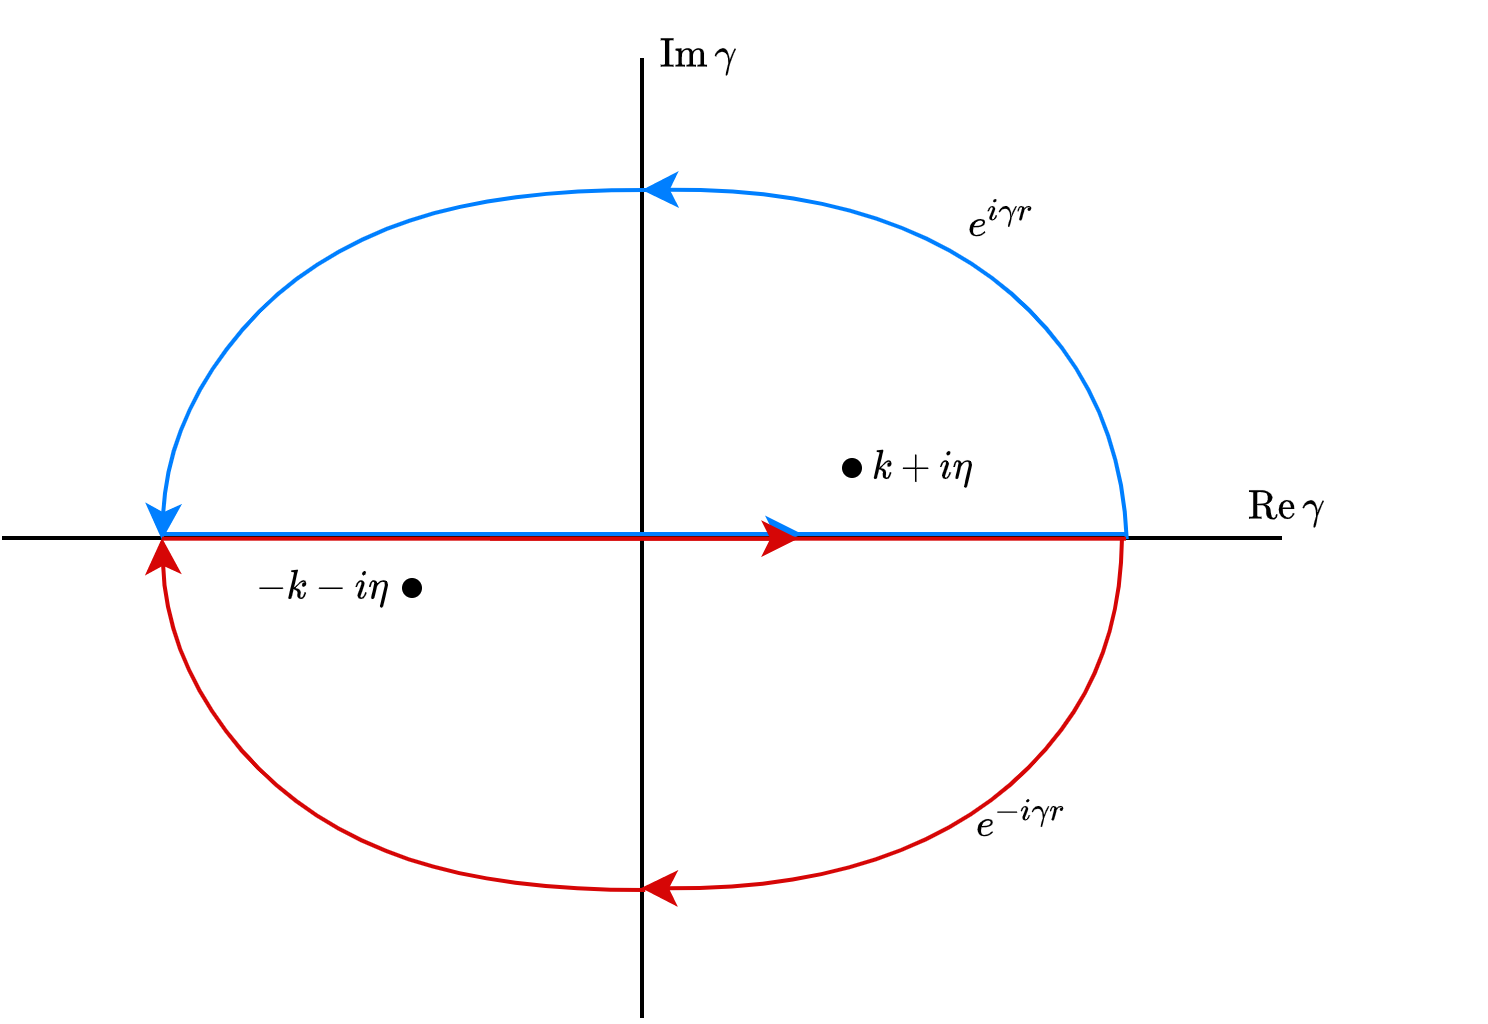
\includegraphics[scale=0.75]{helmholtz_contour.png}
	\caption*{\footnotesize The contours taken to compute the Helmholtz Green's function. The poles are indicated with the assumption $\eta>0$. If instead $\eta<0$, the poles would be flipped over the real axis into the opposite contour.}
\end{figure}
	
	\subsection{The Sommerfeld Radiation Condition}
	It is worth pointing out that a slightly different result is found if the $k$ had been given a negative imaginary part $\eta < 0$ instead. This would flip the poles over the imaginary axis so each of the two contours used would enclose the opposite pole. As a consequence, the end result would have $e^{ -ik r}$ instead of the positive exponent. Considering that the choice of $\eta$ being positive or negative was completely arbitrary, one might wonder if one should be preferred over the other. The interpretation is clearer when the time dependence of the Green's function is included: $G(r,t)=e^{i(kr-\omega t)}/4\pi r$. As $t\to \infty$ an isophase front of $G$ proceeds \emph{outward} $r\to \infty$. When the sign on $k$ is flipped, an \emph{inward} propagating wave is found. Virtually always, we are interested in the outward propagating waves since the source term in the Helmholtz equation should be just that: a \emph{source}, not a sink.
	
	It should not come as a complete surprise that there is some ambiguity in the solution since no boundary conditions have been specified for the problem. So to single out the outward propagating wave, it would be useful to determine a boundary condition at infinity. The correct condition is known as the \textbf{Sommerfeld radiation condition} and it is written
	$$ \lim_{r\to\infty} r(\partial_r - ik)\psi = 0 $$
	The Green's function $G(r)= e^{ikr}/4\pi r$ is easily shown to satisfy this.

	
	\subsection{General Solutions to Helmholtz}
	Suppose we want to solve the inhomogeneous Helmholtz equation with some boundary condition such that
	\begin{align*}
		(\nabla^2 + k^2)\psi &= f \quad\t{ in }\:\Omega\\
		\psi &= \psi_0 \quad\t{in } \partial\Omega 
	\end{align*}
	Alternatively we could specify inhomogeneous boundary conditions on the gradient such that $\nabla\psi = \nabla\psi_0$ on $\partial\Omega$. The method we will outline here can be used to solve either case.
	
	All we need to do is solve the similar problem for the Green's function:
		\begin{align*}
		(\nabla^2 + k^2)G &= \delta \quad\t{ in }\:\Omega\\
		G &= G_0 \quad\t{in } \partial\Omega 
	\end{align*}
	Suppose we have the Green's function. Then with $\psi(\*r) = \int_\Omega d\*r'\;\psi(\*r')\delta(\*r-\*r')$, the delta function can be replaced with the Helmholtz operator acting on the Green's function to write $ \psi = \int_\Omega \psi (\nabla^2  + k^2) G$.	By the definition of $\psi$ as a solution to the inhomogeneous Helmholtz equation, we can make the replacement $k^2\psi=f - \nabla^2\psi$ and split terms into two integrals to write $ \psi =  \int_\Omega f G + \int_\Omega [\psi\nabla^2 G - G\nabla^2\psi] $.
	Finally, using one of Green's identities\footnote{$\int_\Omega \psi\nabla^2 G = \int_{\partial\Omega}\psi\frac{\partial G}{\partial \*n} - \int_\Omega \nabla\psi\cdot\nabla G$}, the second term is found to be equivalent to an integral over just the boundary and we arrive at the useful equation:
	$$ \psi = \int_\Omega fG + \int_{\partial\Omega}\left[\psi\frac{\partial G}{\partial \*n} - G\frac{\partial \psi}{\partial\*n}\right] $$
	where $\frac{\partial\psi}{\partial\*n}\equiv \nabla\psi\cdot\*n$ with $\*n$ the surface normal on the boundary. The first term is the usual convolution of $f$ and $G$ which gives the solution to the inhomogeneous problem. Since the integral on the boundary is, well, on the boundary, we can apply our boundary conditions to obtain a form that does not depend on the unknown $\psi$. Suppose we want to solve the problem with boundary conditions $\psi=\psi_0$ on $\partial\Omega$. In this case, the particular Green's function that is useful is the one with homogeneous boundary condition $G=0$ on $\partial\Omega$. In this case, the formula above simplifies to
	$$ \psi = \int_\Omega f G + \int_{\partial\Omega} \psi_0 \frac{\partial G}{\partial\*n} $$
	which can be computed exactly in principle. Alternatively, if we want to solve the problem with a boundary condition of the form $\frac{\partial\psi}{\partial\*n} = \frac{\partial\psi_0}{\partial\*n}$ on $\partial\Omega$ then the most useful Green's function would be the one which satisfies the analogous homogeneous boundary condition $\frac{\partial G}{\partial\*n} = 0$ on $\partial\Omega$. In this case, the general formula simplifies to
	$$ \psi = \int_\Omega fG - \int_{\partial\Omega} G\frac{\partial\psi_0}{\partial\*n} $$
	Clearly then, this formula provides a very general tool for calculating the solutions to the Helmholtz equation.
	
	\subsection{Kirchoff's Scalar Diffraction Theory}
	The scalar diffraction theory of Kirchoff is entirely based on the previous discussion. In a diffraction problem, we are interested in the electromagnetic field in a region of space with no charges so $\bt{E}$ satisfies the homogeneous Helmholtz equation and our formula leaves\footnote{Notice this implies the field over all $\Omega$ is fully determined by the field at just the boundary $\partial\Omega$. }
	$$ \t{E} = \int_{\partial\Omega}\left[ \t{E}\frac{\partial G}{\partial \*n} - G\frac{\partial \t{E}}{\partial \*n}\right] $$
	To make use of this equation, we must have information about both E$|_{\partial\Omega}$ and $\nabla \t{E}|_{\partial\Omega}$. 
	Kirchoff considered the domain $\Omega$ to be a half space separated from the other half space by a conducting screen punctured by a pinhole. He then imagined that there is an incident wave coming from the other side of the screen which will pass only through the pinhole. In this problem, the boundary of the domain consists of the screen, the pinhole, and the infinite half-dome
	$$ \partial\Omega = \t{hole} + \t{screen} + \t{half-dome} $$
	We will specify a different boundary condition for each part. On the half dome, we want to assume that only outgoing waves will pass leading to the Sommerfeld radiation condition
	$$ \lim_{r\to\infty} r(\partial_r - ik)\t{E} = 0 $$
	Taking the boundary to infinity, this will allow us to ignore the integral over the half-dome and only the screen + hole need to be accounted for.
	
	Naturally most of the field contribution will come from the hole letting the field propagate through. So a simple approach --- and that taken by Kirchoff --- is to set the field and its gradient to zero along the screen. Note that this is not a mathematically sensible thing to do. In general, either the value of the field or the value of its derivative\footnote{or a linear combination as with Robin boundary conditions} can be specified on the boundary but not both. Nonetheless, this approach will prove useful. This leaves only the integral over the hole:
	$$ \t{E} = \int_{\t{hole}}\left[ \t{E}\frac{\partial G}{\partial \*n} - G\frac{\partial \t{E}}{\partial \*n}\right] $$
	To evaluate this, the E-field and its gradient must be known at the hole. With a point source at location $\*r_0$, we compute
	$$ \t{E}(\*r) = \frac{ik}{(4\pi)^2}\int_\t{hole} d\*s  \frac{e^{ik[|\*s - \*r_0| + |\*r - \*s|]}}{|\*s - \*r_0||\*r - \*s|} \left( \cos \theta - \cos\theta_0\right) $$
	where $\theta$ and $\theta_0$ are the angles from $\*s$ to $\*r$ and $\*r_0$ respectively with respect to the inward facing surface normal of the hole.
	
	\section{Sources of Radiation}
	\subsection{Multipole Radiation}
	Consider an arbitrary current distribution $\bt{j}$ oscillating at frequency $\omega$ for which we would like to calculate the fields. Focusing on regions of empty space outside of the source, the vector potential is actually all that is needed. Once $\bt{A}$ is known, the magnetic field is calculated as the curl $\mu_0\bt{H}=\nabla\times\bt{A}$ and then, outside of the source, the Maxwell-Ampere equation gives the electric field through $-i\omega\epsilon_0\bt{E} = \nabla\times\bt{H}$. Recall that in the Lorenz gauge, the vector potential is given by the integral
	$$ \bt{A}(\*r,\omega) = \mu_0\int_{\R^3}d\*r'\;\bt{j}(\*r',\omega)G(|\*r - \*r'|) $$
	where $G(r)=e^{ikr}/2\pi r$ is the Green's function. Supposing that the current density is fully supported in some domain $\Omega$ with characteristic length $L$, we will focus on observation points such that $r\gg L$. Consequently, the integral will be over points where $r'\ll r$ allowing us to make the approximation $|\*r-\*r'| \approx r - \*n\cdot\*r'$. Expanding the Green's function to first order in this approximation gives
	$$ G(r - \*n\cdot\*r') = G(r) - G'(r)\*n\cdot\*r' + \dots $$
	Plugging this into the integral for the vector potential, we find there are two terms $\bt{A} = \bt{A}^{(0)} + \bt{A}^{(1)}$ where
	\begin{align*}
		\bt{A}^{(0)}(\*r,\omega) &= \mu_0G(r)\int_\Omega d\*r'\;\bt{j}(\*r',\omega)\\
 \bt{A}^{(1)}(\*r,\omega) &= - \mu_0G'(r)\int_\Omega d\*r'\;(\*n\cdot\*r')\bt{j}(\*r',\omega)
	\end{align*}

	The zeroth order term $\bt{A}^{(0)}$ is related to the electric dipole moment of the source while the first order term $\bt{A}^{(1)}$ contains contributions from both the magnetic dipole moment and the electric quadrupole moment. We will now calculate these contributions one at at time.
	
	\subsection{Electric Dipole Radiation}

	The zeroth order term contains the integral of the current density over all space. Integrating by parts\footnote{Componentwise: $\int_\Omega \t{j}_x = \int_\Omega \bt{j}\cdot\nabla x = \int_{\partial\Omega} x\bt{j} - \int_\Omega x\nabla\cdot\bt{j}$} and using the fact that the current distribution is finite and vanishes on the boundary $\partial\Omega$, this can be shown to be equal to
	$$ \int_\Omega d\*r'\;\bt{j}(\*r',\omega) = -i\omega \bt{d}(\omega) $$
	Indeed, this follows from the continuity equation in the frequency domain $\nabla\cdot\bt{j}=i\omega\rho$ which introduces the charge density $\rho$ and the integral is exactly the dipole moment. In fact, the whole term $-i\omega\bt{d}$ is understood in the time domain as the derivative of the dipole moment. The zeroth order expression for the vector potential is therefore
	$$ \bt{A}^{(0)}(\*r,\omega) = -i\omega \mu_0 G(r)\bt{d} $$
	To calculate the fields from this, we start with the H-field computed with the curl $\bt{H}^{(0)} = \nabla\times \bt{A}^{(1)}/\mu_0$. With a useful (and easily derived) curl identity\footnote{For radial $\psi=\psi(r)$: $ \nabla\times \psi\*V = \psi'\,\*n\times\*V + \psi \nabla\times\*V $}, this is obtained as
	$$ \bt{H}^{(0)}(\*r,\omega) = -i\omega G'(r)\*n\times\bt{d} $$
	With the H-field in hand, the corresponding E-field can be computed from $-i\omega\epsilon_0\bt{E}^{(0)}=\nabla\times\bt{H}^{(0)}$ using the same vector calculus identity:
	\begin{align*}
		\epsilon_0\bt{E}^{(0)}(\*r,\omega) &= G''(r)\*n\times(\*n\times\bt{d}) \\
		 & \:+ G'(r)\nabla\times(\*n\times\bt{d})
	\end{align*}
	At this point, we can insert the relevant Green's function derivatives
\begin{align*}
	G'(r) &= -G(r)\frac{1-ikr}{r} \\
	G''(r)&= G(r) \left[ \frac{2(1 - ikr)}{r^2} - k^2 \right]
\end{align*}
	Along with another curl identity that is found without too much trouble using another vector formula\footnote{The triple product formula: $\*a\times(\*b\times\*c) = (\*c\cdot\*a)\*b - (\*a\cdot\*b)\*c$}:
	$$ \nabla\times(\*n\times\*d) = -\frac{(\*n\*n^\t{T} + \mathbbm{1})\bt{d}}{r}$$
	Putting these results together we obtain an explicit equation for the fields. However, it is worth including one additional step where the $2(1-ikr)/r^2$ term in $G''(r)$ is rewritten with 	$ \*n\times(\*n\times\*d) = (\*n\*n^\t{T} - \mathbbm{1})\bt{d} $. This allows us to group terms of the appropriate falloff and obtain the complete result. So finally, the full H and E fields from the electric dipole contribution are given by\sidenote{Electric dipole radiation fields}
	\begin{multline*} 
	\bt{E}^{(0)}(\*r,\omega) = \frac{e^{ikr}}{4\pi\epsilon_0}\bigg[\frac{1-ikr}{r^3}(3\*n\*n^\t{T} - \mathbbm{1})\bt{d}\\ + \frac{k^2}{r}(\*n\times\bt{d})\times\*n \bigg] 
	\end{multline*}
	$$ \bt{H}^{(0)}(\*r,\omega) = i\omega\frac{e^{ikr}}{4\pi }\frac{1-ikr}{r^2}\*n\times\bt{d} \qquad\qquad\quad\quad $$
	These equations have many features worth pointing out. First, observe that in the static limit $\omega\to 0$, the E-field reduces to exactly the static dipole field and the H-field vanishes as expected. Also observe that in the far field where $kr\gg 1$, the lowest order terms in $1/r$ dominate and we obtain the following fields:
	\begin{align*}
		\bt{E}^{(0)}(\*r, \omega) &\sim \frac{e^{ikr}k^2}{4\pi\epsilon_0 r} (\*n\times\bt{d})\times\*n \\
		\bt{H}^{(0)}(\*r,\omega) &\sim \frac{e^{ikr}ck^2}{4\pi r} \*n\times\bt{d}
	\end{align*}
	This exhibits the relationship $\bt{E}^{(0)} = \eta_0 \bt{H}^{(0)}\times \*n$ where $\eta_0=1/c\epsilon_0=\sqrt{\mu_0/\epsilon_0}$ is the impedance of free space. Notice that these equations imply that the electric field, magnetic field, and the radial direction $\*n$ form an orthogonal triad. The Poynting vector points radially.
	$$ \bt{S}^{(0)} = \frac{e^{ikr}ck^4d^2}{(4\pi)^2\epsilon_0r^2}\*n $$
	
	\subsection{Magnetic Dipole Radiation}
	
	Now turning to $\bt{A}^{(1)}$, we will write it again here for convenience:
	$$  \bt{A}^{(1)}(\*r,\omega) = - \mu_0G'(r)\int_\Omega d\*r'\;(\*n\cdot\*r')\bt{j}(\*r',\omega) $$
	This term is best understood by splitting the integrand into symmetric and antisymmetric parts such that
	$$ (\*n\cdot\*r')\bt{j} = \underbrace{\frac{(\*n\cdot\*r')\bt{j} + (\*n\cdot\bt{j})\*r'}{2}}_{\t{even}} + \underbrace{\frac{(\*n\cdot\*r')\bt{j} - (\*n\cdot\bt{j})\*r'}{2}}_{\t{odd}} $$
	The resulting two terms for the vector potential $ \bt{A}^{(1)} = \bt{A}^{(1e)} + \bt{A}^{(1o)}$ will turn out to be related to the electric quadrupole and magnetic dipole moment respectively. We will first focus on the magnetic dipole contribution. Indeed, the odd part can be immediately simplified with the same vector triple product identity used previously to find the magnetic dipole moment: $ \t{odd part } = \bt{m}\times\*n $ where $\bt{m}=\frac{1}{2}\int d\*r'\; (\*r'\times\bt{j})$. So the odd part of the vector potential here is
	$$ \bt{A}^{(1o)} = -\mu_0 G'(r)\bt{m}\times\*n $$
	Computing the magnetic field from this is exactly the same calculation that we carried out to get the electric dipole E-field from its H-field. We need only map $\bt{d}\mapsto \bt{m}$. So the H-field for the magnetic/odd term is immediately obtained this way. 	The E-field can also be immediately found by invoking $\bt{E}=-\nabla\phi +i\omega\bt{A}$. Since there is no first order contribution to the scalar potential from the magnetic dipole, this reduces to $\bt{E}^{(1o)}=i\omega\bt{A}^{(1o)}$. So then, we obtain the fields with little extra work: \sidenote{Magnetic dipole radiation fields}
	\begin{multline*} 
	\bt{H}^{(1o)}(\*r,\omega) = \frac{e^{ikr}}{4\pi}\bigg[\frac{1-ikr}{r^3}(3\*n\*n^\t{T} - \mathbbm{1})\bt{m}\\ + \frac{k^2}{r}(\*n\times\bt{m})\times\*n \bigg] 
\end{multline*}
	$$ \bt{E}^{(1o)}(\*r,\omega) = -i\omega \mu_0\frac{e^{ikr}}{4\pi}  \frac{1-ikr}{ r^2}\*n\times\bt{m} \qquad\:\quad$$
	In the static limit $\omega\to 0$, the H-field reduces to exactly the static magnetic dipole field and the E-field vanishes as expected. In the far field, we recover the radiated fields
	\begin{align*}
	\bt{H}^{(1o)}(\*r, \omega) &\sim \frac{e^{ikr}k^2}{4\pi r} (\*n\times\bt{m})\times\*n \\
	\bt{E}^{(1o)}(\*r,\omega) &\sim -\frac{e^{ikr}\mu_0 ck^2}{4\pi r} \*n\times\bt{m}
\end{align*}
	which imply the same orthogonal triad relationship between E-field, H-field, and the radiated direction $\*n$ as found for the electric dipole (thanks to the minus sign in the E-field here).
	
	\subsection{Electric Quadrupole Radiation}
	Now the even part is most easily dealt with by looking at it componentwise. The integral is
	$$ \t{A}_i^{(1e)}(\*r,\omega) = -\frac{\mu_0}{2}G'(r)\int_\Omega d\*r'\;(\t{j}_i x_j' + x_i'\t{j}_j)n_j $$
	Observing that $\t{j}_i = \bt{j}\cdot\nabla x_i$, the integrand can be rewritten using $\t{j}_i x_j' + x_i'\t{j}_j = \bt{j}\cdot\nabla(x_i'x_j')$. Then integrating by parts\footnote{$\int_\Omega \bt{j}\cdot\nabla(x_i'x_j') = \int_{\partial\Omega} d\*\sigma\cdot\bt{j}x_i'x_j' - \int_\Omega x_i'x_j' \nabla\cdot\bt{j}$} and using the fact that $\bt{j}$ is localized to a finite region of space, this becomes 
	$$ \int_\Omega d\*r'(\t{j}_i x_j' + x_i'\t{j}_j)n_j = -i\omega\int_\Omega d\*r'\;\rho(\*r')x_i'x_j' n_j $$
	where we have used the continuity equation $\nabla\cdot\bt{j}=i\omega\rho$ to write the integral in terms of, what is evidently, the quadrupole moment of the charge distribution. Recall that the traceless quadrupole moment is defined by $Q_{ij} = \int \rho(3 x_ix_j - \delta_{ij}r^2)$ so the \emph{primitive moment} which appears in the above expression is related through $\int \rho x_ix_j = \frac{1}{3}[Q_{ij} + \delta_{ij}\int \rho r^2 ]$. The additional term added to the quadrupole moment can be ignored since it will appear in the final expression for the vector potential as parallel to $\*n$ and will therefore vanish when we take the curl. With that, the first order even term for the vector potential is
	$$ \bt{A}^{(1e)}(\*r,\omega) = \frac{i\omega\mu_0}{6} G'(r) Q\*n $$
	To now compute the H-field, the curl is computed using the same familiar curl identity we have used previously. Noting that $\nabla\times Q\*n =-\*n\times Q\*n/r$, the radiated magnetic field from the quadrupole moment is
$$ \bt{H}^{(1e)}(\*r,\omega) = \frac{i\omega}{6}\left[G''(r) - \frac{G'(r)}{r}\right]\*n\times Q\*n$$
	Now to get the E-field, we cannot use the same trick as before with $\bt{E}=i\omega\bt{A}$ and the full curl must be computed instead. Once again using the same curl identity as before, we have
	\begin{multline*} 
		\bt{E}^{(1e)} = \frac{-1}{6\epsilon_0}\bigg[\left[G'''(r) - \frac{G''(r)}{r} + \frac{G'(r)}{r^2}\right]\*n\times(\*n\times Q\*n) \\
		+ \left[G''(r) - \frac{G'(r)}{r}\right] \nabla\times(\*n\times Q\*n)\bigg]
	\end{multline*}
	The remaining curl to compute is
	$$ \nabla\times(\*n\times Q\*n) = -\frac{(2\*n\*n^\t{T} + \mathbbm{1})Q\*n}{r} $$
	Taking the appropriate derivatives gives
	\begin{multline*} 
	\bt{E}^{(1e)} = \frac{G(r)}{6\epsilon_0}\left[ik^3 - \frac{4k^2}{r} + \frac{9(1-ikr)}{r^3}\right]\*n\times(\*n\times Q\*n) \\
	+ \frac{G(r)}{6\epsilon_0}\left[\frac{3(1-ikr)}{r^3} - \frac{k^2}{r}\right] (2\*n\*n^\t{T} +\mathbbm{1})Q\*n
\end{multline*}
	At this point, we can rearrange terms to make this more understandable. Similar to what we did for the electric dipole fields, we will use the convenient identity $\*n\times(\*n\times Q\*n)=(\*n\*n^\t{T}-\mathbbm{1})Q\*n$ to combine the $1/r^4$ terms as well as the $1/r^2$ terms. As a consequence, the static quadrupole field will fall out naturally. Indeed, we can recast the above equation to arrive at the final form for the electric quadrupole fields:\sidenote{Electric quadrupole radiation fields}
	\begin{multline*} 
	\bt{E}^{(1e)} = \frac{e^{ikr}}{24\pi\epsilon_0}\bigg[ \frac{3}{r^4} (5\*n\*n^\t{T} - 2)Q\*n \\
	-\frac{2k^2}{r^2}(3\*n\*n^\t{T} - \mathbbm{1})Q\*n\\
	+ \frac{ik^3}{r} \*n\times(\*n\times Q\*n) \bigg] 
\end{multline*}
	$$ \bt{H}^{(1e)}(\*r,\omega) = \frac{i\omega e^{ikr}}{24\pi}\left[\frac{3(1 - ikr)}{r^3} - \frac{k^2}{r} \right]\*n\times Q\*n $$
	As mentioned, we can see that in the static limit, the H-field disappears and the E-field reduces to exactly the static electric quadrupole field. On the other hand, in the far field where $kr\gg 1$, we recover the following radiation fields:
	\begin{align*}
		\bt{H}^{(1e)} &\sim -\frac{ick^3 e^{ikr}}{24\pi r} \*n\times Q\*n \\
		\bt{E}^{(1e)} &\sim -\frac{ik^3}{24\pi \epsilon_0 r} (\*n\times Q\*n)\times\*n
	\end{align*}
	Notice that these fields scale with frequency as $k^3$ as compared to the dipole terms which scale as $k^2$. This suggests that higher order multipole fields will radiate more strongly at higher frequencies. 
	
	\section{Plane Waves}
	\subsection{Properties of EM Plane Waves}
	$$ \bt{E}(\*r,t) = \bt{E}_0 e^{i(\*k\cdot\*r - \omega t)} $$
	where $\t{E}_{0x}, \t{E}_{0y}, \t{ and } \t{E}_{0z}$ are the complex components of the field, each having their own magnitude and phase. 
	\subsection{Linear, Circular, \& Elliptical Polarization}
	Since the far field E and H fields satisfy the orthogonality condition $\*n \propto \*E\times\*H$, the fields must be entirely \textbf{transverse}, polarized only in the plane orthogonal to the direction of propagation. In this plane, we define the polarization vector
	$$ \*\psi = \begin{pmatrix}
		\cos\frac{\theta}{2} \\
		e^{i\phi}\sin\frac{\theta}{2}
	\end{pmatrix} = \cos\frac{\theta}{2}\ket{+} + e^{i\phi}\sin\frac{\theta}{2}\ket{-} $$
	
	\subsection{Reflection \& Refraction}
	\subsection{The Fresnel Equations}
	
	\section{Scattering}
	\subsection{Scattering from Perfect Conductors}
	Recall the inhomogeneous equation for the E-field
	$$ -(\nabla^2\bt E + k^2 \bt{E}) = -\frac{\nabla\rho}{\epsilon_0} - i\omega \mu_0 \bt j  $$
	The contrinuity equation is $i\omega\nabla\rho = -\nabla(\nabla\cdot\bt{j})$.
	$$	(\nabla^2 + k^2) \bt{E} = i\omega \mu_0 \left[ \bt{j} +  \frac{\nabla(\nabla\cdot\bt{j})}{k^2} \right]$$
	This has solution in terms of the Green's function
	$$ \bt{E}(\*r,\omega) = i\omega\mu_0 \int_\Omega d\*r'\;G(|\*r-\*r'|) \left[ \bt{j} +  \frac{\nabla'(\nabla'\cdot\bt{j} )}{k^2} \right] $$

	\subsection{Babinet's Principle}
	\subsection{Small Obstacles}
	\subsection{Born Approximation}
	\subsection{Partial Wave Analysis}
	
	\section{Relativity \& Covariant EM}
	\subsection{Lorentz Transformations}
	Electrodynamics is intimately related to special relativity. Consider the homogeneous wave equation 
	$$ \left[-\nabla^2 + \frac{1}{c^2}\frac{\partial^2}{\partial t^2}\right]\psi = 0 $$
	We want to find the set of transformations which leave this equation invariant. We will consider a general coordinate transformation in space and time so that the new coordinates are $\*s'=\Lambda\*s$ where $\*s=(ct,\*r)$. The gradient with respect to these spacetime coordinates is $\partial = (\frac{1}{c}\partial_t, \nabla)$. The wave equation can be written in terms of this spacetime gradient as 
	$$ g^{\mu\nu}\partial\mu \partial_\nu = 0 $$
	where we have defined the \textbf{Minkowski metric} $g = \t{diag}(-1,1,1,1)$.
	\subsection{Tensors}
	\subsection{Covariant Maxwell's Equations}
	The Faraday tensor is 
	$$ F_{\mu\nu} = \partial_\mu A_\nu - \partial_\nu A_\mu $$
	$$ \partial_\mu F^{\mu\nu} = \mu_0 j^\nu $$
	$$ \partial_\mu F_{\nu\lambda} + \partial_\nu F_{\lambda\mu} + \partial_\lambda F_{\mu\nu}= 0 $$
	
	
	\newpage
	\appendix
	\section{Green's Identities}
	Green's (first) identity is just a multivariable version of integration by parts. We begin with the the divergence theorem which is written for a differentiable vector field $\*F:\R^3\to \R^3$ and a volume $\Omega\subset\R^3$:
	$$ \int_\Omega \nabla\cdot \*F = \oint_{\partial\Omega}d\*\sigma\cdot\*F $$
	With $\*F=\psi\*\Gamma$, this is
	$$ \int_\Omega \nabla\cdot(\psi\*\Gamma) = \oint_{\partial\Omega}d\*\sigma\cdot\*\Gamma \psi $$
	The divergence term is easily calculated in index notation to be $\nabla\cdot \psi\*\Gamma = \partial_i(\psi \Gamma_i)= \partial_i\psi \Gamma_i + \psi \partial_i\Gamma_i$. So moving terms around, we find
	$$ \int_\Omega \psi \nabla\cdot\*\Gamma = \oint_{\partial\Omega} d\*\sigma\cdot\*\Gamma \psi - \int_\Omega \nabla\psi\cdot\*\Gamma $$
	Observe that this is just like the standard integration by parts formula $\int_\Omega udv = uv\big|_{\partial\Omega} - \int_\Omega vdu$



\end{document}